\documentclass[convert = false, tikz]{standalone}
\usepackage[utf8]{inputenc}
\usepackage{tikz}
\usetikzlibrary{automata, positioning, arrows}
 
% \usepackage{../../../../style_automata}

% arara: pdflatex
% arara: latexmk: { clean: partial }

\begin{document}
    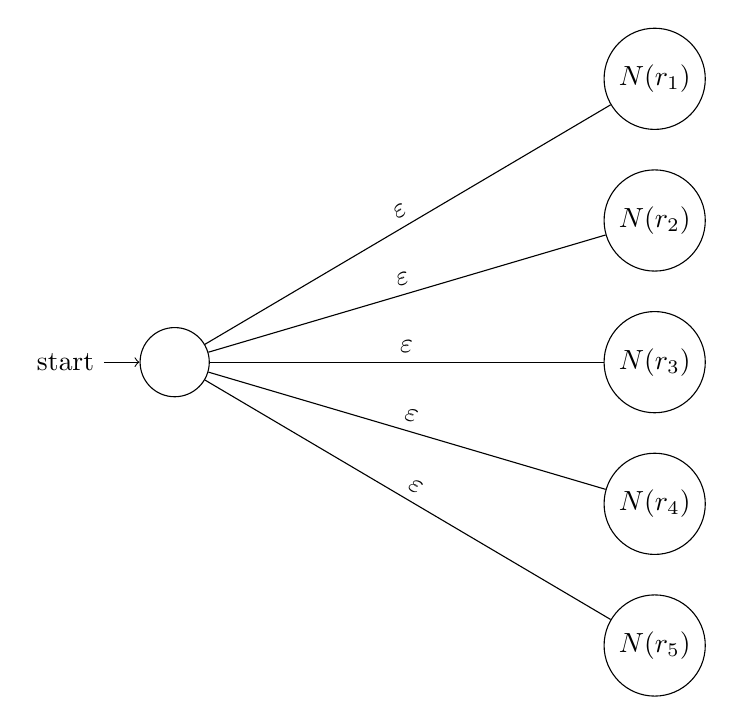
\begin{tikzpicture}
        \begin{scope}
            % start node
            \node (0) [state, initial] {};

            % other nodes
            \node [state, right = 5cm of 0] (3) {$N(r_3)$}; % fuck off latex
            \node [state, above = 5mm of 3] (2) {$N(r_2)$};
            \node [state, above = 5mm of 2] (1) {$N(r_1)$};
            \node [state, below = 5mm of 3] (4) {$N(r_4)$};
            \node [state, below = 5mm of 4] (5) {$N(r_5)$};
            

            % edges
            \draw (0) -- node[above,sloped] {$\varepsilon$} (1);
            \draw (0) -- node[above,sloped] {$\varepsilon$} (2);
            \draw (0) -- node[above,sloped] {$\varepsilon$} (3);
            \draw (0) -- node[above,sloped] {$\varepsilon$} (4);
            \draw (0) -- node[above,sloped] {$\varepsilon$} (5);
        
        \end{scope}
    \end{tikzpicture}
\end{document}
